In questo capitolo viene introdotta una panoramica sulla struttuazione dell’architettura del servizio affinché possano essere soddisfatte le esigenze illustrate nel capitolo precedente.

Problematiche di questo tipo vengono risolte tramite lo sviluppo di un’applicazione web, o webApp cioè un'applicazione accessibile via web per mezzo di un network (es. una Intranet o la Rete Internet). Trattasi di un modello applicativo di elevata comodità, in quanto permette ad ogni utente di effettuare una consultazione interattiva delle informazioni di cui necessita.

Una webApp è strutturata su tre livelli: il primo livello è associabile al terminale di fruizione, il web browser; il secondo livello è costituito dal motore applicativo (core applicativo)  formato da codice sorgente in un qualche linguaggio di sviluppo dinamico lato-server (in questo caso Java); il terzo livello è riconducibile alla conservazione ed estrapolazione dei dati di interesse, cosicché possano essere riutilizzati in qualsiasi momento.

Una volta noto il funzionamento delle applicazioni web, per lo sviluppo di questo servizio si è scelto di utilizzare, come di consuetudine tra gli sviluppatori web, lo schema architetturale MVC.

Infine le risorse vengono definite e indirizzate tramite il REpresentational State Transfer (REST) cioè un tipo di architettura software per i sistemi di ipertesto distribuiti


\section{La Struttura Server-Client} % (fold)
\label{sec:la_struttura_server_client}

% section la_struttura_server_client (end)

% section section_name (end)

Per una webApp è necessaria un’architettura Server-Client, formata cioè da due parti ben distinte che comunicano attraverso un linguaggio ad esse comune.

Per far si che l’applicazione sia semplice da utilizzare ed accessibile alla maggior parte dell’utenza, è necessario che il progetto relativo al lato Client sia ben strutturato affinché sia facile la ricerca delle informazioni da parte dell’utente. E gestisca in maniera efficiente la mole di dati inviati dal Server.

Il Client, per sua natura, non compie operazioni complesse ma si limita a richiedere i dati di cui necessita, al server, per fornirne la visualizzazione. 

Il Server è l’entità complessa che gestisce tutta la mole di dati che servono affinché l’applicazione funzioni. Esso ha il compito di: ricevere le richieste del client, prelevare i dati da un gestore esterno o da un’altra fonte, trattarli opportunamente secondo la richiesta ricevuta e restituirli nella forma richiesta.

Secondo quanto sopra, è facilmente intuibile come il server si trovi a gestire un’elevata mole di dati e lo deve fare riducendo al minimo i tempi di attesa. Sono necessarie, quindi, performance elevate.

\newpage


\section{Applicazioni web: one page application} % (fold)
\label{sec:applicazioni_web_one_page_application}

Per comprendere il sistema che è alla base di questa architettura, si forniscono degli esempi. Essi partono da interazioni Cliet-Server di vecchio modello e arrivano a quelle di nuova generazione facendo notare la loro evoluzione. In un sito web tradizionale, l’esperienza dell’utente verrebbe trattata semplicemente facendo uso di una serie di reindirizzamenti come si può vedere dalla figura n.1 sotto riportata:

\begin{figure}[htbp]
\begin{center}
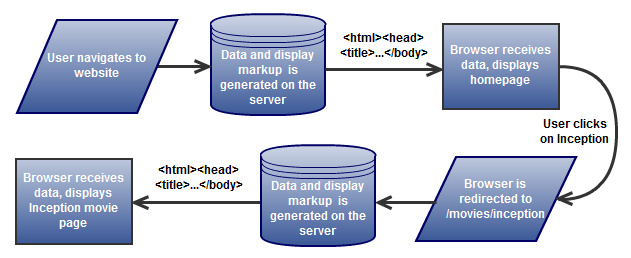
\includegraphics{contents/images/web_app_flow_2_1_}
\end{center}
\caption{}
\label{fig:flow_0}
\end{figure}

L’utente, tramite Client, accede al sito web; il server riceve e processa la richiesta ricevuta, genera i dati, li elabora se richiesto, e li invia con l’HTML necessario al client che, una volta ricevute le informazioni le elabora e consente la visualizzazione. A questo punto l’utente è in condizioni di navigare liberamente cercando quello di cui ha bisogno tenendo presente, però, che ad ogni singola richiesta corrisponde una nuova elaborazione, da parte del server, che dovrà generare nuovi dati, elaborati o non, per restituirli con l’HTML al client che verrà reindirizzato sulla pagina richiesta.
\newpage
Un’applicazione web di nuova generazione, ossia one page application, invece, previene qualsiasi reindirizzamento non necessario e permette la visualizzazione di diverse richieste in un’unica pagina, rendendo l’esperienza dell’utente molto più fluida e veloce come dalla figura n. 2 sotto riportata:

\begin{figure}[htbp]
\begin{center}
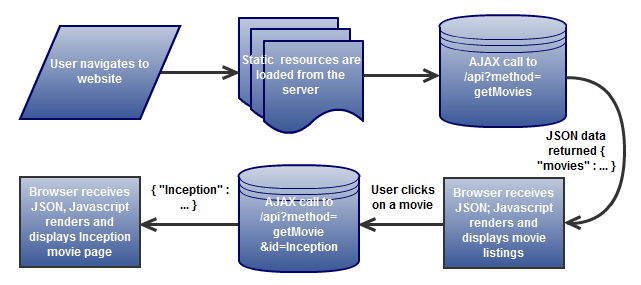
\includegraphics{contents/images/web_app_flow_3_1_}
\end{center}
\caption{}
\label{fig:flow_1}
\end{figure}

Qui, l’utente, tramite Client, accede al sito web ma, in questo caso, il server non elabora dati, né genera l’HTML, si limita a trasmette al browser tutte le risorse necessarie affinché possano essere elaborate per la creazione dei differenti aspetti della pagina. A questo punto inizia la navigazione dell’utente, il client invia le richieste al server tramite chiamate asincrone di tipo AJAX ed esso, processando quanto richiesto, restituirà solamente le informazioni che interesano. E’ compito del client occuparsi della visualizzazione corretta di quanto ricevuto utilizzando le risorse già in suo possesso.

Da questa breve trattazione si può notare come l’utilizzo di un’applicazione web di ultima generazione incrementi notevolmente la reattività del servizio. In queste webApp il carico di lavoro, non grava più esclusivamente sul server, ma viene ripartito tra i due lati. Questo permette al server di occuparsi della gestione dei dati e lascia tutti i compiti di presentazione al browser, che da semplice visualizzatore diventa, a tutti gli effetti, uno strumento attivo per la costruzione delle strutture di rappresentazione dei dati.

\newpage

\section{Il pattern MVC} % (fold)
\label{sec:il_pattern_mvc}

Una volta noto il funzionamento delle applicazioni web, per lo sviluppo di questo servizio si è scelto di utilizzare, come di consuetudine tra gli sviluppatori web, lo schema architetturale MVC.
MVC si basa sul concetto di applicazione basata su tre livelli: Model, View e Controller illustrato nella figura seguente:

\begin{figure}[htbp]
\begin{center}
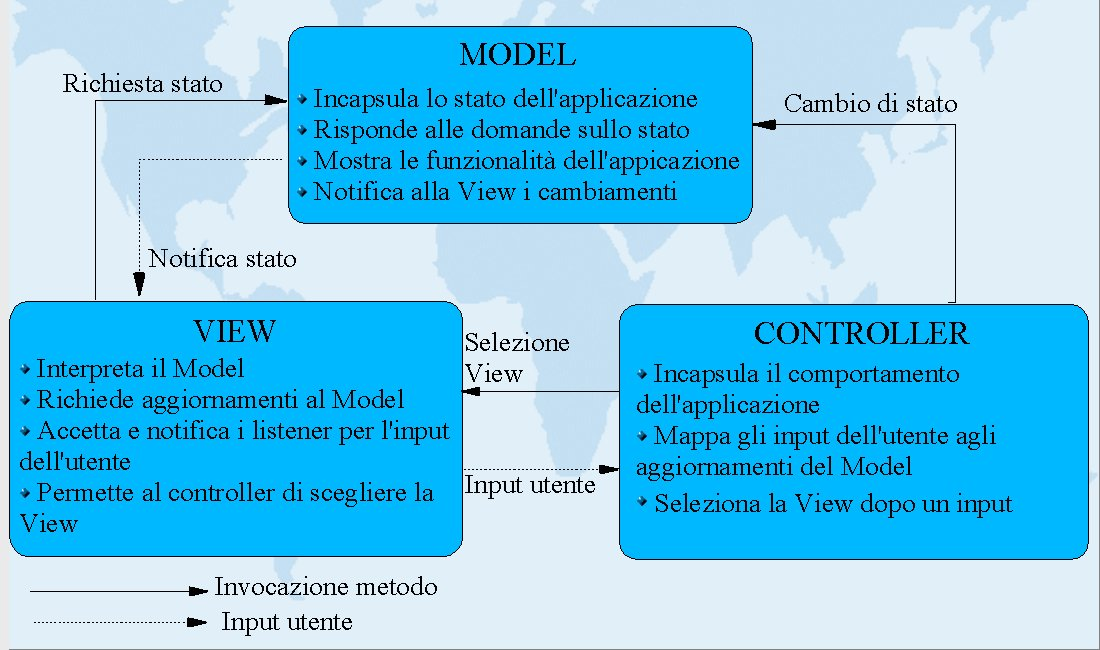
\includegraphics[width=10cm]{contents/images/mvc}
\end{center}
\caption{}
\label{fig:mvc}
\end{figure}



Il Model (modello) rappresenta lo strato che si occupa di fornire i metodi per l’accesso e la gestione dei dati primitivi (consultazione, modifica e salvataggio)  e la notifica alla View dei vari cambiamenti di stato.
Lo strato View (vista) si occupa solamente della metodologia di visualizzazione dei dati forniti dal modello per presentare, in maniera chiara e comprensibile, una rappresentazione dell’informazione.
Il Controller (controllore) ha il ruolo di ricevere i comandi dell’utente e formulare, di conseguenza, un’azione che risponda alle sue esigenze.
Quando l’utente formula una richiesta, il Controller si occupa di manipolare, attraverso dei comandi, i dati conservati nello strato Model. A seguito del cambiamento dei dati nel Model, lo strato View aggiornerà la loro rappresentazione in tempo reale. Concluso questo ciclo, potrà avere subito inizio una nuova richiesta. 
Utilizzando questo schema architetturale è possibile disaccoppiare e diminuire la coesione tra le varie componenti principali di un’applicazione che può essere esportata su qualsiasi piattaforma, al massimo dovrà essere rivisto il livello View per l’adattamento ai vari tipi di interfaccia grafica. 
L’esportazione di un’applicazione che non rispetta questo schema comporta il rifacimento dell’intera applicazione dovuta ad una elevata coesione della componente grafica verso tutte le altre impedendone l’uso. 

\section{Direttive REST} % (fold)
\label{sec:direttive_rest}

REpresentational State Transfer (REST) è un tipo di architettura software per i sistemi di ipertesto distribuiti come il World Wide Web e  si riferisce ad un insieme di principi di architetture di rete, i quali delineano come le risorse sono definite e indirizzate. I 5 principi fondamentali di questo tipo di architettura sono:
\begin{itemize}
    \item Il sistema deve essere necessariamente costituito da due parti ben distinte: Server-Client che interagiscono con interfacce comuni
    \item Il sistema deve essere stateless, ossia non si deve essere legati al fatto di dovere tenere aperte delle sessioni differenti da utente a utente. Quindi ogni richiesta fatta da ogni client può essere processata dal Server indipendentemente dalle richieste precedenti. Questo vincolo non impedisce però al Server di mantenere una cache di alcuni dati per migliorare le prestazioni e i tempi di risposta.
    \item Il sistema deve essere in grado di supportare una cache a diversi livelli. I browser commerciali sono in grado di eseguire il caching delle informazioni inviate dai vari server disponibili in Internet. Pertanto le risposte devono, implicitamente o esplicitamente, definire i livelli consentiti di cache al fine di supportare il client nell’ottimizzazione consistente delle performance.
    \item I sistemi devono essere accessibili in modo uniforme: ogni risorsa deve avere un indirizzo univoco globale e un punto valido di accesso. Ciò definisce un’interfaccia uniforme che permette un elevato grado di disaccoppiamento tra client e server.
    \item Il sistema deve essere stratificato. Un client internet normalmente non è in grado di determinare se è connesso direttamente con il server o se è connesso attraverso un agente intermedio.
    \item Questo è un vincolo facoltativo: i sistemi coinvolti devono essere in grado di estendere temporaneamente o di personalizzare le funzionalità al lato client attraverso il trasferimento di codice eseguibile. Alcuni esempi sono dati dal trasferimento di componenti eseguibili come le applet Java o di script sorgenti come JavaScript.
\end{itemize}

L’architettura REST permette oggi di avere servizi Web scalabili, efficienti e raggiungibili da chiunque ed ovunque. Seguendo questi principi di ha la possibilità di testare il funzionamento di un’applicazione per mezzo di un semplice browser commerciale. Ciò è particolarmente utile anche durante le fasi iniziali di implementazione dell’integrazione.

\newpage
